\scanpage{136}
\deleted{Position de}\quad +\quad Les relations
\[
\underset{\mathcal G^{+!}}{\underset{\Vert}{\Pi}}\simeq
\underset{\mathcal G_0^{+!}}{\underset{\Vert}{\Pi_0}}\times\{\pm1\},\quad
\Pi'=\{1,\tau\}\cdot\Pi=D_\tau\cdot\Pi_0=\Pi'_0\times\mu
\]
\[
\Pi'_0=\{1,\tau\}\cdot\Pi_0
\]
\textcircled{II}
\diagram{\begin{tikzcd}[row sep=large,column sep=large]
\mu_\tau \arrow[rr,hook,"2"] \arrow[dr,hook,"2"] & & D_\tau=\mu_\tau\times\mu \arrow[dr,hook,"2"] & & & \\
& \mathcal G_0^!=\Pi'_0 \arrow[rr,hook,"2"] & & \Pi'=\Pi'_0\times\mu=\mathcal G^! \arrow[rr,hook,no head,"6"] \arrow[ddrrr,hook] & & \mathcal G \arrow[ddrr,hook] & & \\
\{1\} \arrow[uu,hook,"2"] \arrow[rr,hook,"2"] \arrow[dr,hook,"2"] & & \underline\mu \arrow[uu,hook,"2"] \arrow[dr,hook,"2"] & & & & & & \\
& \mathcal G_0^{+!}=\Pi_0 \arrow[uu,hook,"2"] \arrow[rr,hook,"2"] & & \Pi=\Pi_0\times\mu=\mathcal G^{+!} \arrow[uu,hook,"2"] \arrow[rr,hook,"6"] \arrow[ddrr,hook] & & \mathcal G^+ \arrow[uu,hook,"2"] \arrow[ddrrr,hook] & \mathcal M^! \arrow[r,"6"] & \mathcal M & {}\\
& & & & & & & & \\
& & & & & \mathcal M^{+!} \arrow[uur,hook,"\widehat{\mathbb Z}^{*}\deleted{\unsure{2}}"] \arrow[rrr,hook,"6"] & & {}& \mathcal M^+ \arrow[uul,hook,"\widehat{\mathbb Z}^{*}\deleted{\unsure{2}}"]
\end{tikzcd}}

\diagram{\begin{tikzcd}[row sep=large]
\Pi_0\simeq\{\lambda_0,\lambda_1,\lambda_\infty\mid\lambda_\infty\lambda_1\lambda_0=1\} \arrow[d,hook]\\
\mathcal G
\end{tikzcd}}
\[
\lambda_i\longmapsto-\ell_i
\]

\diagram{\begin{tikzcd}[row sep=large,column sep=large]
& \deleted{\mathcal M^!} \arrow[rr] & & \deleted{\mathcal M}\\
\deleted{\Pi'=\mathcal G^!} \arrow[ur,hook] \arrow[rr,hook] & & \deleted{\mathcal G} \arrow[ur,hook] & \\
& \deleted{\mathcal M^{+!}} \arrow[uu,hook] \arrow[rr] & & \deleted{\mathcal M^+} \arrow[uu,hook]\\
\deleted{\mathcal G^{+!}} \arrow[uu,hook] \arrow[ur,hook] \arrow[rr,hook] & & \deleted{\mathcal G^+} \arrow[uu,hook] \arrow[ur,hook] &
\end{tikzcd}}
\figure{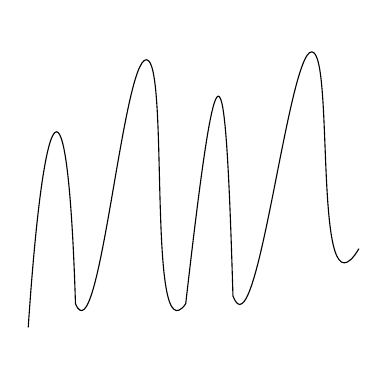
\begin{tikzpicture}\draw (0,0) .. controls (.2,3) and (.5,3.5) .. (.6,.3) .. controls (.9,-.4) and (1.2,3.4) .. (1.5,3.4) .. controls (1.8,3.4) and (1.5,-.4) .. (2,.3) .. controls (2.4,3.8) and (2.5,3.8) .. (2.6,.4) .. controls (2.9,-.4) and (3.3,3.5) .. (3.6,3.5) .. controls (3.9,3.5) and (3.6,0) .. (4.2,1);\end{tikzpicture}}

$\mathcal G/\Pi_0$ ou $\mathcal G^+/\Pi_0$ déduits de $\mathcal G$ \unsure{et|ou} $\mathcal G^+$ en divisant par la relation $\tau'(\rho)=\deleted{\unsure{\rho}}\sigma(\rho)$ ou encore $\tau(\rho)=\rho$ ($\uline{\mathrm{NB}}\ \tau(\rho)=\deleted{\unsure{1}}-(\ell_{\unsure{i|1}}^{-1})\rho$ !)

\rule{\linewidth}{0.4pt}
\uline{III}\quad\deleted{position de $\mathcal M(0)$}

$\mathcal M(0)$ et groupes associés

\diagram{\begin{tikzcd}[column sep=large,row sep=large]
\mathcal M(0) \arrow[r,hook] & \unsure{\mathcal M^\Pi_\Pi[0]|\mathcal M^\Pi[0]} \arrow[rr,hook] \arrow[dr,hook,"6"] & & \mathcal M^! \arrow[dr,hook] & \\
& & \mathcal M^{\mathcal G}[0] \arrow[rr,hook] & & \mathcal M \arrow[dd,dash]\\
\mu_\tau \arrow[uu,hook] \arrow[r,hook] & D_0^\Pi \arrow[uu,hook] \arrow[rr,hook] \arrow[dr,hook,"2"] & & \Pi'=\mathcal G^! \arrow[uu,hook] \arrow[dr,hook] & \\
& & D_0^{\mathcal G} \arrow[uu,hook] \arrow[rr,hook] & & \mathcal G\\
\{1\} \arrow[uu,hook] \arrow[r,hook,"\widehat{\mathbb Z}"] & L_0^\Pi \arrow[uu,hook] \arrow[rr,hook] \arrow[dr,hook,"2"] & & \underline\Pi=\mathcal G^{+!} \arrow[uu,hook] \arrow[dr,hook,"6"] & \\
& & L_0^{\mathcal G} \arrow[uu,hook] \arrow[rr,hook] & & \mathcal G^+ \arrow[uu,hook,no head]
\end{tikzcd}}

\diagram{\begin{tikzcd}[column sep=large,row sep=large]
{} \arrow[dr,dash,gray] & & \\
& L_0^{\Pi_0} \arrow[r,dash,gray] & {}
\end{tikzcd}}
\margin{136}
